% Options for packages loaded elsewhere
\PassOptionsToPackage{unicode}{hyperref}
\PassOptionsToPackage{hyphens}{url}
%
\documentclass[
  9pt,
  ignorenonframetext,
]{beamer}
\usepackage{pgfpages}
\setbeamertemplate{caption}[numbered]
\setbeamertemplate{caption label separator}{: }
\setbeamercolor{caption name}{fg=normal text.fg}
\beamertemplatenavigationsymbolsempty
% Prevent slide breaks in the middle of a paragraph
\widowpenalties 1 10000
\raggedbottom
\setbeamertemplate{part page}{
  \centering
  \begin{beamercolorbox}[sep=16pt,center]{part title}
    \usebeamerfont{part title}\insertpart\par
  \end{beamercolorbox}
}
\setbeamertemplate{section page}{
  \centering
  \begin{beamercolorbox}[sep=12pt,center]{part title}
    \usebeamerfont{section title}\insertsection\par
  \end{beamercolorbox}
}
\setbeamertemplate{subsection page}{
  \centering
  \begin{beamercolorbox}[sep=8pt,center]{part title}
    \usebeamerfont{subsection title}\insertsubsection\par
  \end{beamercolorbox}
}
\AtBeginPart{
  \frame{\partpage}
}
\AtBeginSection{
  \ifbibliography
  \else
    \frame{\sectionpage}
  \fi
}
\AtBeginSubsection{
  \frame{\subsectionpage}
}
\usepackage{lmodern}
\usepackage{amsmath}
\usepackage{ifxetex,ifluatex}
\ifnum 0\ifxetex 1\fi\ifluatex 1\fi=0 % if pdftex
  \usepackage[T1]{fontenc}
  \usepackage[utf8]{inputenc}
  \usepackage{textcomp} % provide euro and other symbols
  \usepackage{amssymb}
\else % if luatex or xetex
  \usepackage{unicode-math}
  \defaultfontfeatures{Scale=MatchLowercase}
  \defaultfontfeatures[\rmfamily]{Ligatures=TeX,Scale=1}
\fi
\usetheme[]{Goettingen}
\usecolortheme{rose}
% Use upquote if available, for straight quotes in verbatim environments
\IfFileExists{upquote.sty}{\usepackage{upquote}}{}
\IfFileExists{microtype.sty}{% use microtype if available
  \usepackage[]{microtype}
  \UseMicrotypeSet[protrusion]{basicmath} % disable protrusion for tt fonts
}{}
\makeatletter
\@ifundefined{KOMAClassName}{% if non-KOMA class
  \IfFileExists{parskip.sty}{%
    \usepackage{parskip}
  }{% else
    \setlength{\parindent}{0pt}
    \setlength{\parskip}{6pt plus 2pt minus 1pt}}
}{% if KOMA class
  \KOMAoptions{parskip=half}}
\makeatother
\usepackage{xcolor}
\IfFileExists{xurl.sty}{\usepackage{xurl}}{} % add URL line breaks if available
\IfFileExists{bookmark.sty}{\usepackage{bookmark}}{\usepackage{hyperref}}
\hypersetup{
  pdftitle={BIOS6643 Longitudinal},
  pdfauthor={EJC},
  hidelinks,
  pdfcreator={LaTeX via pandoc}}
\urlstyle{same} % disable monospaced font for URLs
\newif\ifbibliography
\setlength{\emergencystretch}{3em} % prevent overfull lines
\providecommand{\tightlist}{%
  \setlength{\itemsep}{0pt}\setlength{\parskip}{0pt}}
\setcounter{secnumdepth}{-\maxdimen} % remove section numbering
\AtBeginSubsection{}
\AtBeginSection{}
\ifluatex
  \usepackage{selnolig}  % disable illegal ligatures
\fi

\title{BIOS6643 Longitudinal}
\subtitle{L21 Nonparametric}
\author{EJC}
\date{}
\institute{Department of Biostatistics \& Informatics}

\begin{document}
\frame{\titlepage}

\begin{frame}[allowframebreaks]
  \tableofcontents[hideallsubsections]
\end{frame}
\hypertarget{nonparametric-regression}{%
\section{Nonparametric regression}\label{nonparametric-regression}}

\begin{frame}{Topics for this lecture:}
\protect\hypertarget{topics-for-this-lecture}{}
\begin{itemize}
\tightlist
\item
  Nonparametric regression - local polynomial regression
\end{itemize}

\vspace{\baselineskip}

\begin{itemize}
\item
  Associated reading:

  \begin{itemize}
  \tightlist
  \item
    Section 3 of the `Nonparametric and flexible longitudinal
    regression' notes.
  \end{itemize}
\end{itemize}
\end{frame}

\hypertarget{longitudinal-nonparametric-regression}{%
\section{Longitudinal nonparametric
regression}\label{longitudinal-nonparametric-regression}}

\begin{frame}{Local polynomial regression and other nonparametric
regression techniques}
\protect\hypertarget{local-polynomial-regression-and-other-nonparametric-regression-techniques}{}
Various techniques for longitudinal nonparametric regression have been
developed recently. Many of these techniques have been developed by
adding mixed model elements to existing nonparametric regression
methods. One source for the following information is Wu (2006).

Some common nonparametric regression techniques include local polynomial
regression (LOESS), spline modeling (e.g., regression, smoothing and
penalized splines), and generalized additive models (GAMs).
\end{frame}

\begin{frame}{}
\protect\hypertarget{section}{}
GAMs are in the class of semi-parametric regression models that allow
fitting of both parametric and nonparametric terms.

Spline modeling involves joining regression segments together into one
continuous function. Basics of spline modeling were presented in
previous notes. In the context of nonparametric regression, spline
modeling often involves more knots.

LOESS regression is essentially carried out by performing weighted
polynomial regression about a focal point \(x_0\), where the weights are
determined as a function of \(x-x_0\), with smaller values getting
higher weight (i.e., the closer \(x\) is to \(x_0\), the higher the
weight). The local regression at \(x_0\) produces an estimated \(y\) at
the point \(x_0\), which is just the intercept value of the fitted
function. This process is then repeated across other focal points to
yield a smooth function.
\end{frame}

\begin{frame}{}
\protect\hypertarget{section-1}{}
In LOESS regression (or local polynomial regression), the function that
defines the weighting structure is called the kernel.

For example, we could use a standard normal kernel:
\(f(u)=\frac 1 {\sqrt {2\pi}} e^{-u^2 /2}\), where \(u=(x-x_0)/h\) and
\(h\) is called the bandwidth, which helps determine the smoothness of
the fitted function (the higher the value, the smoother the fit). As the
equations indicate, higher weight is given to values closer to \(x_0\),
and then drop for values of \(x\) that are further from \(x_0\).

An even simpler approach is to use a uniform kernel, which will give
equal weight to values in the local regression about x\_0, but will only
include a certain percentage of all data values.
\end{frame}

\begin{frame}{}
\protect\hypertarget{section-2}{}
Another common approach is to use a hybrid of both of these approaches:
use the tricube function (somewhat similar in shape to the normal), but
then only include the nearest fixed percentage of values to \(x_0\),
i.e., a truncated tricube function (see Figure 1 for shape). In this
case, the tricube function is standardized and the control over the
smoothness is determined by the percentage of values used in the local
regression, sometimes referred to as the span or smoothing parameter.

There are a variety of methods that can be used to select optimal
bandwidths for a given data set, including \(AIC_C\), \(AIC_{C1}\) and
generalized cross validation (GCV) statistics. SAS Help describes these
under PROC LOESS documentation. Bandwidth selection is important because
not only will it determine the smoothness of the fit, it plays a strong
role in the degree of bias and variance in the associated estimators.
\end{frame}

\begin{frame}{}
\protect\hypertarget{section-3}{}
The degree of the polynomial is usually between 0 and 3, but more
commonly 1 (local linear regression) or 2 (local quadratic regression).
You might be wondering: if you only use the fitted intercept, then why
even bother with higher order terms? The main reason is that it reduces
bias in the estimated function. Specifically, it allows you to use a
larger bandwidth (producing a smoother function) without inducing as
much bias as you would have for lower order polynomials.

Figure 1 illustrates how LOESS regression works using Fox's Occupational
Prestige data. Panels (a)-(c) demonstrate the local regression at
\(x_0=8000\) to produce \(\hat y_{x=8000}\); panel (d) is the complete
fit by performing multiple local fits across \(x\).
\end{frame}

\begin{frame}{}
\protect\hypertarget{section-4}{}
\begin{center}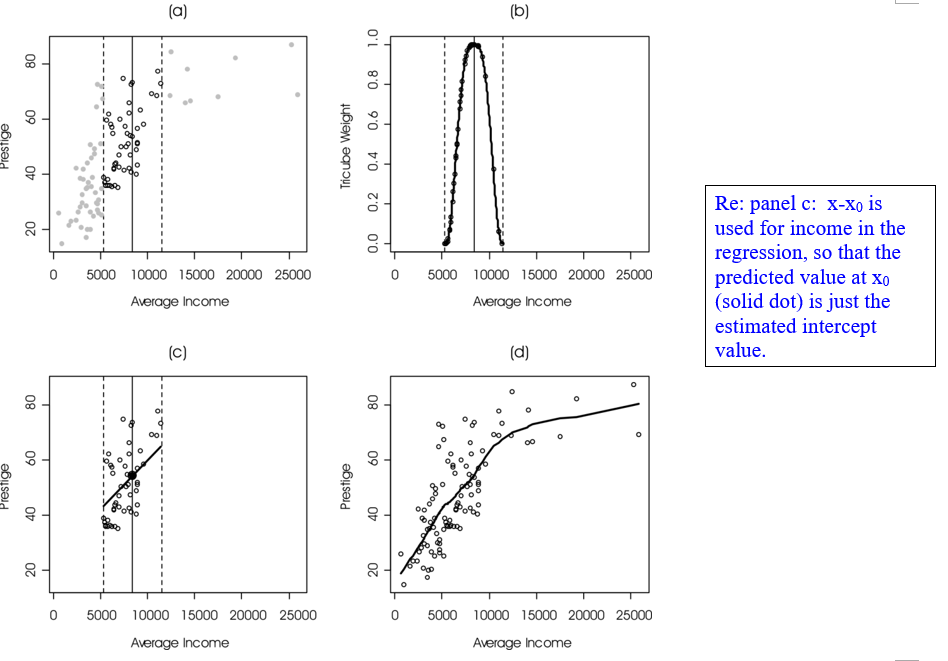
\includegraphics[width=0.5\linewidth]{figs_L21/f1} \end{center}
\end{frame}

\begin{frame}{}
\protect\hypertarget{section-5}{}
Figure 1 (from Fox, 2000): Local linear regression of prestige on income
for the 1971 Canadian occupational-prestige data:

\begin{enumerate}
\tightlist
\item
  The broken lines delimit the 50 nearest neighbors of \(x_0 = \$8403\)
  (the 80th ordered \(x\) value, at the solid vertical line).
\item
  Tricube weights for observations in the neighborhood of \(x_0\).
\item
  Locally weighted linear regression in the neighborhood of \(x_0\); the
  solid dot is the fitted value above \(x_0\).\\
\item
  The completed locally linear regression, connecting fitted values
  across the range of \(x\).
\end{enumerate}

In Figure 1, the kernel/bandwidth method used was the hybrid method,
with use of the tricube kernel but then only using the 50 nearest
neighbors to \(x_0\) in the local regression (span=49\%, as n=102).
\end{frame}

\hypertarget{longitudinal-nonparametric-regression-1}{%
\section{Longitudinal nonparametric
regression}\label{longitudinal-nonparametric-regression-1}}

\begin{frame}{Longitudinal nonparametric regression}
\protect\hypertarget{longitudinal-nonparametric-regression-2}{}
Nonparametric regression can be augmented to account for longitudinal
data. One basic approach is to incorporate mixed model elements while
fitting, and thus account for the correlated nature of longitudinal
data.

Adding mixed model elements to GAM yields Generalized Additive Mixed
Models (GAMMs), which allow for modeling of longitudinal data for
various types of outcomes (e.g., normal, binomial, Poisson).

Wood (2006) is one good resource for GAMMs. Wu (2006) discusses adding
mixed model elements into spline modeling and LOESS regression, yielding
mixed-effect spline modeling and local polynomial mixed-effects
regression, respectively. Here we will primarily focus on the latter.
\end{frame}

\begin{frame}{Statistical models for longitudinal nonparametric
regression}
\protect\hypertarget{statistical-models-for-longitudinal-nonparametric-regression}{}
Before discussing local mixed regression, let's consider the
nonparametric functions that we are interested in estimating. There are
two basic types that we will consider here. One is a nonparametric
population mean model, and one is a nonparametric mixed-effects models.

Consider data (\(t_ij\), \(y_ij\)), \(i=1,\ ...,\ N\),
\(j=1,\ ...,\ n_i\), where \(t_ij\) is the \(j\)th time point
observation for subject \(i\). These data can be used to fit either the
nonparametric population mean (NPM) model:
\(Y_i(t) = \eta (t)+\epsilon _i (t) \ \ \ \ (1)\). Or the nonparametric
mixed-effects model (NPME) model:
\(Y_i(t)= \eta(t)+ v_i(t)+\epsilon _i(t) \ \ \  \ (2)\) where time
(\(t\)) is modeled as a continuous variable, \(\eta (t)\) is a
fixed-effect function for the population mean, \(v_i(t)\) represents the
departure of the \(i\)th individual from the population mean function
(the random effect function for subject \(i\)), and \(\epsilon_i(t)\) is
the error function for subject \(i\). The mean function for the
population is \(\eta (t)\) and the mean function for subject \(i\) is
\(\eta (t) + v_i(t)\).
\end{frame}

\begin{frame}{}
\protect\hypertarget{section-6}{}
A common approach to fit (1) is to use mixed-effect spline models; (2)
can be fit using local polynomial mixed-effect modeling. Note that the
population mean term, \(\eta (t)\), and subject deviation term,
\(v_i(t)\), are smooth functions that are not constrained by any
parametric form. However, when fitting these terms with nonparametric
regression, you can get smoother or less smooth functions by controlling
bandwidth parameters.
\end{frame}

\begin{frame}{Local polynomial mixed-effect modeling}
\protect\hypertarget{local-polynomial-mixed-effect-modeling}{}
We can fit (2) by using the same local regression techniques as LOESS,
but fitting a weighted mixed model instead of weighted least squares
regression model. This will allow us to get estimates for both
\(\eta (t)\) and \(v_i(t)\), for \(i=1,\ ...,\ n\).

For example, \(Y\) may represent some type of growth data (e.g.,
height), \(\eta (t)\) is the population height function of time, and
\(v_i(t)\) is the (true) height function for subject \(i\). When we
estimate \(\eta (t)\) using nonparametric regression (call it
\(\hat \eta (t)\)), we end up with a growth estimate for each \(t\) that
cannot be summarized by simple regression coefficients.

Thus, we usually graph \(\hat \eta(t)\) as a function of \(t\). The main
strength of NP regression is that we are not forcing the data to be
constrained by a particular parametric function, which often
over-summarize the growth characteristics over time. The main drawback
is that we do not end up with a set of regression coefficients that
summarize the growth curve.
\end{frame}

\begin{frame}{}
\protect\hypertarget{section-7}{}
Before carrying out the nonparametric mixed-effect modeling, we need to
determine the optimal bandwidth to use. The added complexity here
relative to LOESS for independent data, is that the best bandwidth for
the population mean function may not be the same as for the
subject-specific functions.

There are a variety of suggested methods to use to select bandwidth.
Simpler approaches include using cross validation statistics and more
complex methods include backfitting algorithms (see Wu text for
details). A leave-one-subject out cross validation (SCV) can be used to
select the best bandwidth for the population mean fit, while a
leave-one-point out cross validation statistic (PCV) can be used for
optimal subject specific functions. The lowest values of these
statistics indicate optimal bandwidths for the population mean and
subject offsets, respectively.

Then one can the local fit using the optimal bandwidth as indicated by
the SCV statistic to estimate \(\eta (t_0)\), use a separate local fit
using the optimal bandwidth as indicated by the PCV statistic to
estimate \(v_i(t_0)\), and combine these to get the subject-specific
estimate.

Now we have doubled the number of PROC MIXED fits necessary to carry out
the NP longitudinal regression! Although this seems like a lot, the
newer backfitting algorithm suggested by Wu is even more computer
intensive.
\end{frame}

\hypertarget{application}{%
\section{Application}\label{application}}

\begin{frame}{FEV1 of students with moderate to severe asthma}
\protect\hypertarget{fev1-of-students-with-moderate-to-severe-asthma}{}
FEV1 of students with moderate to severe asthma at the Kunsberg School
at NJH were monitored over approximately 7 months during the 2003-04
school year. The optimal bandwidths as indicated by the SCV and PCV
statistics were approximately 25 and 30, respectively. Since the values
were fairly close, each local fitting was carried out with the bandwidth
of 30 only.

Figure 2: Illustration of fit of a nonparametric mixed-effects model for
FEV1 data obtained from children attending the Kunsberg School at NJH
during the 2003-04 school year. The population mean fit,
\(\hat \eta (t)\) is the bold line; fits for two of the 43 subjects
(\(\hat \eta (t)+\hat v_i(t)\)) are given with dashed lines with their
actual data superimposed (subject with higher FEV1 with closed circles;
subject with lower FEV1 with open circles).
\end{frame}

\begin{frame}{}
\protect\hypertarget{section-8}{}
\begin{center}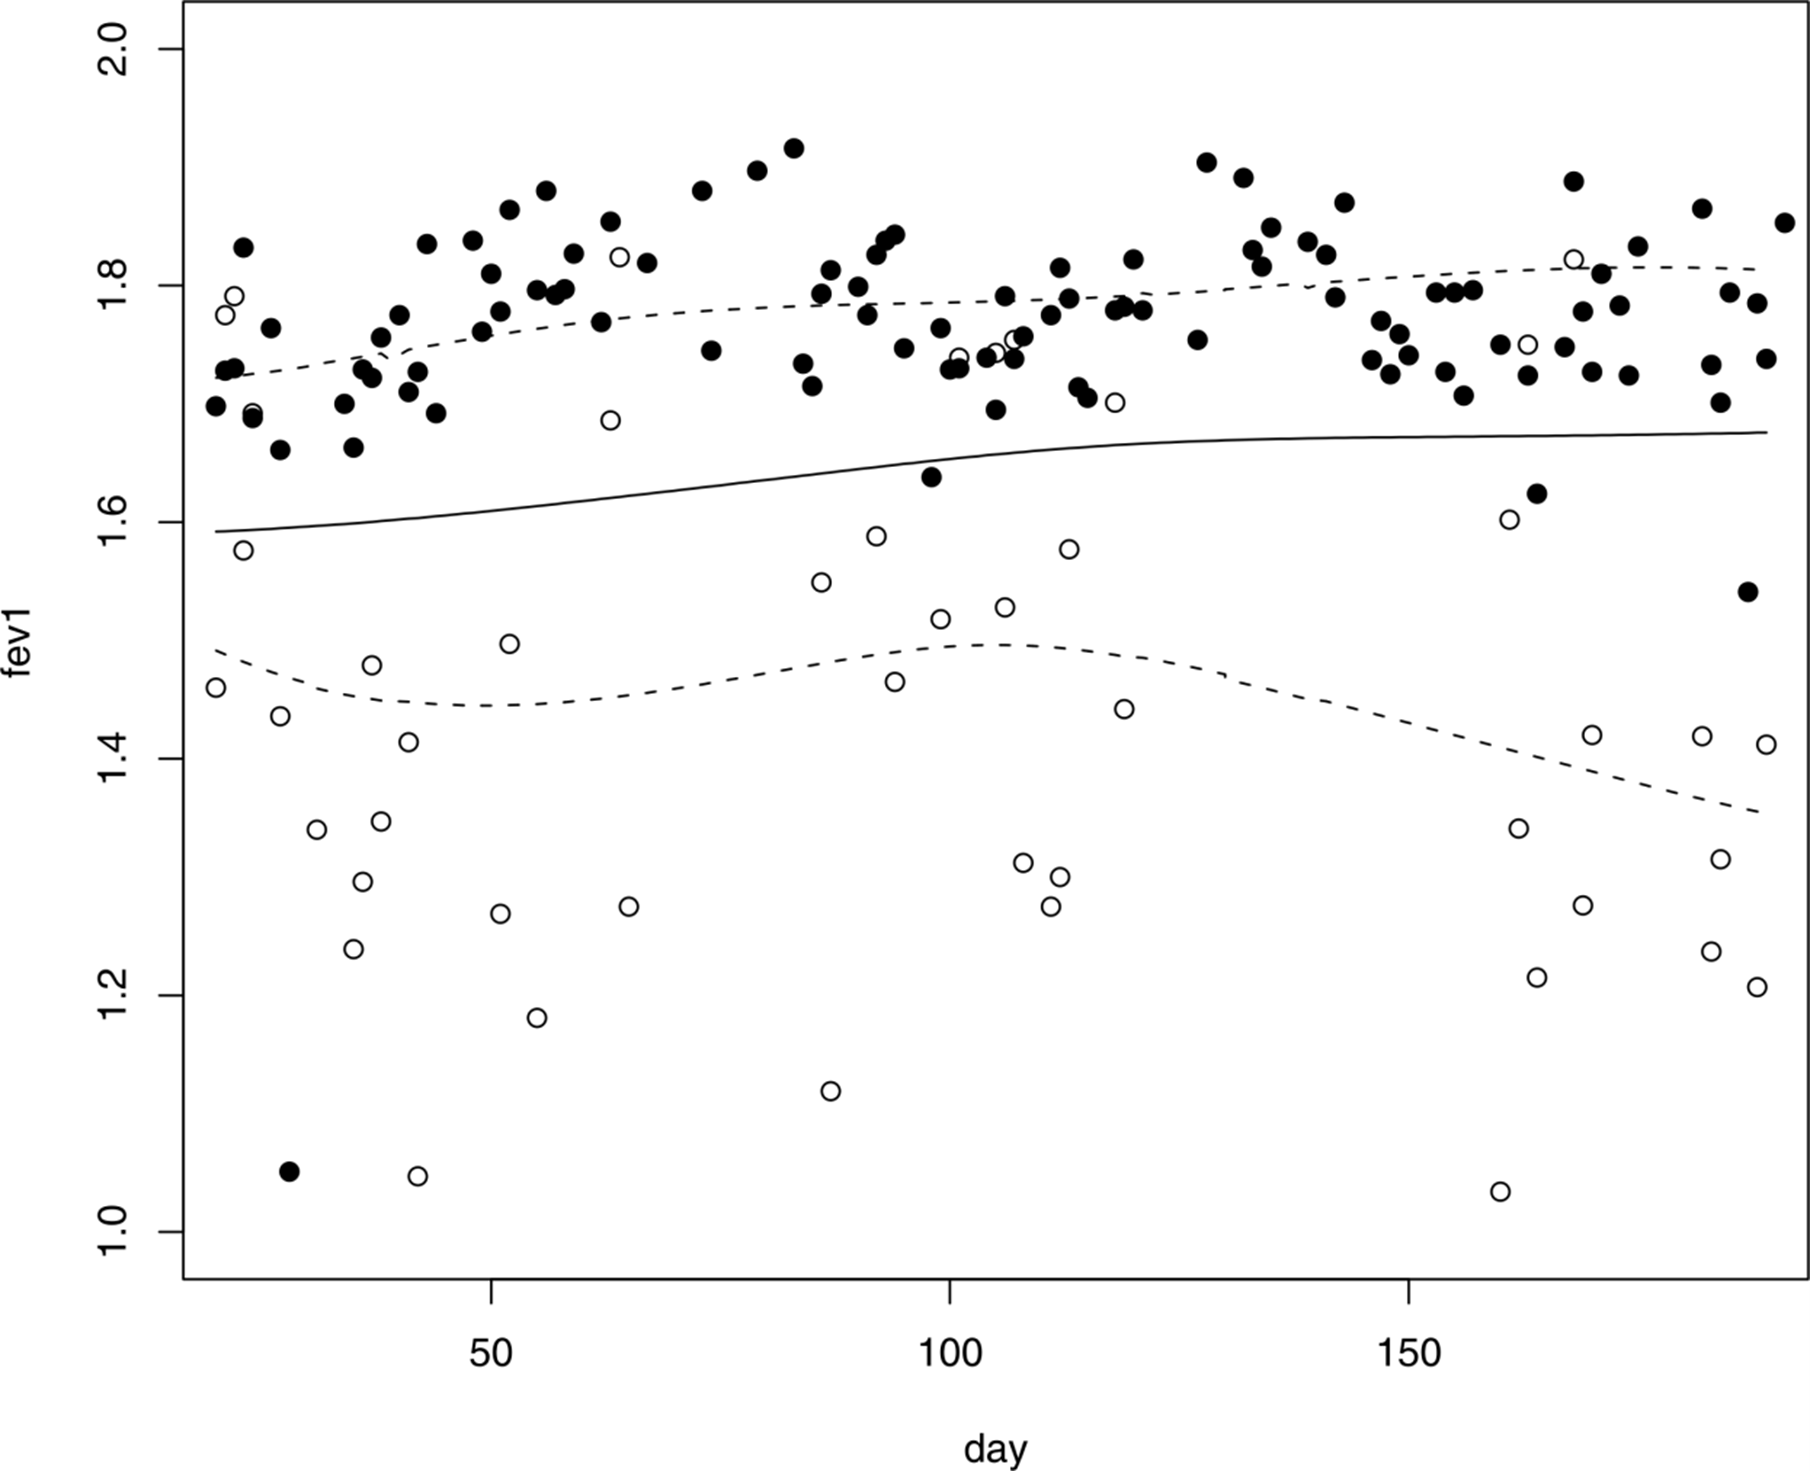
\includegraphics[width=0.7\linewidth]{figs_L21/f2} \end{center}
\end{frame}

\begin{frame}{}
\protect\hypertarget{section-9}{}
The fit demonstrates how flexible the nonparametric fit is. The
population mean estimate increases steadily during the study period (as
expected), but more so in the first half.

Subject 346 (with higher values) has a trend that is similar to the
population mean estimate trend. However, subject 427 (lower) clearly
does not follow this trend; this subject seems to drop down in the
second half of the study.

Variations from the slight growth can occur for certain subjects if they
start to struggle with their asthma (e.g., seasonal allergies), or have
a period of illness. The next step would be to construct confidence
intervals for \(\eta (t)\) and \(v_i(t)\).

We are currently working on methods of inference for local mixed
regression. In order to carry out the local mixed regression, we need to
perform a mixed model fit across all days. The fit for one such day
(day=30) is given below, with condensed output.
\end{frame}

\begin{frame}{}
\protect\hypertarget{section-10}{}
\begin{center}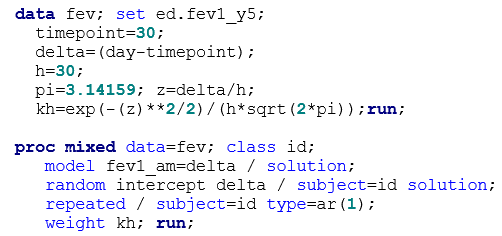
\includegraphics[width=0.6\linewidth]{figs_L21/f3} \end{center}

\begin{center}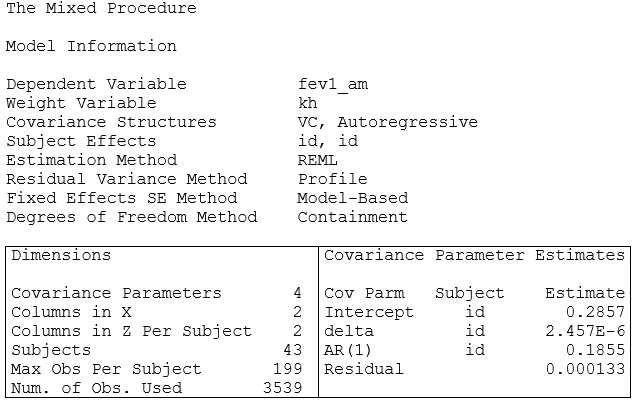
\includegraphics[width=0.6\linewidth]{figs_L21/f4} \end{center}
\end{frame}

\begin{frame}{}
\protect\hypertarget{section-11}{}
\begin{center}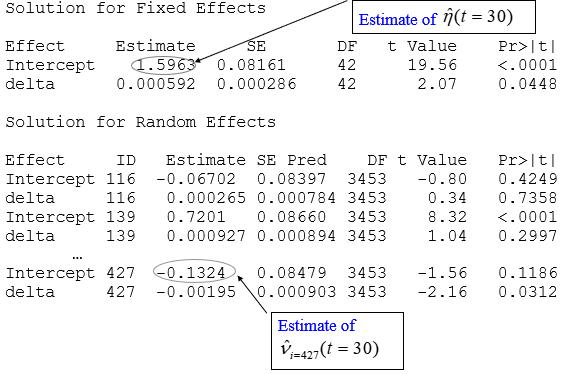
\includegraphics[width=0.6\linewidth]{figs_L21/f5} \end{center}

\begin{center}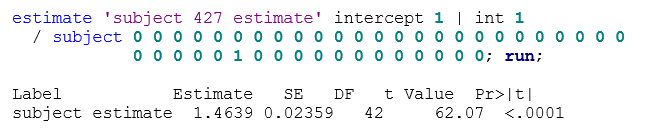
\includegraphics[width=0.6\linewidth]{figs_L21/f6} \end{center}

Based on the mixed model output, the estimated population mean FEV1
estimate at day 30 is 1.5963. The offset for subject 427 is -0.1324.
Combining these can be done in SAS by adding the following statement to
the PROC MIXED code that yields the subsequent output:

The estimate can be matched from above (1.5963 - 0.1324 = 1.4639); the
associated SE of the estimate is much smaller (0.02359) than that of the
individual components which may not be so intuitive and implies that
fixed and random intercept estimates are negatively correlated.
(Requires some further study!)
\end{frame}

\begin{frame}{}
\protect\hypertarget{section-12}{}
Similar fits can be performed across values of time to yield a smooth
mean population function as well as fits for individuals. The data set
for the local fit above specified \(x_0\) = 30. If we stack all such
data sets (one for each \(x_0\)=1 to 199), then we can run one PROC
MIXED and use the BY statement to identify the \(x_0\). Generally, using
the BY statement is more efficient than performing the fits in a loop.
\end{frame}

\begin{frame}{}
\protect\hypertarget{section-13}{}
Nonparametric mixed effect modeling is clearly more computationally
intensive than performing a standard mixed model fit for a parametric
function.

\begin{itemize}
\item
  For these data, there are 199 separate mixed model fits (one for each
  day); you can then double that if you are using different bandwidths
  for population mean and subject specific estimates.
\item
  This may have been a big deal even up to 5 or 10 years ago, but faster
  computers have made this much less of an issue.
\item
  Some computational difficulties may arise if the researcher needs to
  use resampling techniques for methods of inference (e.g., confidence
  intervals), or simulations, but even then may be able to carry out
  computations in a reasonable time if the data sets are not too large.
\item
  For more detail about local mixed modeling and this specific FEV1
  application, please see Ed Hess's Master's Thesis (from our
  Biostatistics Department, 2010).
\end{itemize}
\end{frame}

\hypertarget{references}{%
\section{References}\label{references}}

\begin{frame}{References}
\protect\hypertarget{references-1}{}
Fox, John. Multiple and Generalized Nonparametric Regression. Sage
University Paper, 2000.

Hess, Ed. Non-parametric mixed effect modeling of lung function data.
Master's Thesis, Department of Biostatistics, Colorado School of Public
Health, UCD, July, 2010.

Wood, Simon. Generalized Additive Models: An Introduction with R.
Chapman \& Hall, 2006.

Wu H, Zhang J-T. Nonparametric regression methods for longitudinal data
analysis. Wiley, 2006.
\end{frame}

\hypertarget{summary}{%
\section{Summary}\label{summary}}

\begin{frame}{Summary}
\protect\hypertarget{summary-1}{}
\end{frame}

\end{document}
